% called by main.tex
%
\chapter{Estado del arte}
\label{ch::capitulo2}

\section{Detección de somnolencia}
La detección de somnolencia se divide en dos áreas principales, las cuales están directamente relacionadas con la manera en la que se mide la somnolencia, objetivas y subjetivas.

Las mediciones subjetivas se realizan principalmente a través de observaciones dependientes del sujeto de prueba, donde los individuos reportar su propio nivel de alerta o somnolencia utilizando alguna de las ya establecidas escalas de alerta y somnolencia. Entre las más utilizadas se encuentra la Karolinska Sleepiness Scale (KSS), Epworth Sleepiness Scale (ESS) y Standford Sleepiness Scale. Esta manera de medir la somnolencia presenta una opción sencilla y fácil de utilizar para clasificación (\cite{osamaSubyObj}). 

Gracias a la posibilidad de clasificación numérica, el uso de redes neuronales es muy sencillo con mediciones subjetivas, por lo que se han creado múltiples bases de datos que utilizan esta forma de medición con el objetivo de entrenar redes neuronales y clasificar niveles de somnolencia en base a imagenes del rostro o cuerpo del conductor. Entre las bases de datos más utilizadas se encuentran DROZY, UTA-RLDD, y MCDD, que ofrecen distintos fondos de imagen, ángulos y participantes con los cuales entrenar un modelo de inteligencia artificial (\cite{DrowsyDG}).

La Tabla \ref{tab:subjetivas} muestra la experimentación realizada en el estado del arte que busca predecir somnolencia en un conductor con clasificaciones subjetivas, es decir, escalas como la KSS. Debido a la facilidad de clasificar estas escalas, los métodos utilizados son distintos clasificadores de aprendizaje profundo y aprendizaje automático, obteniendo resultados mixtos, con un rango de exactitudes de 62.84\% a 99.1\%. Se utilizan todo tipo de métricas en la medición de estos clasificadores, como métricas relacionadas al vehículo y al rostro, como el PERCLOS, bostezos, y movimiento de cabeza. 

\begin{table}[h!]
    \centering
    \footnotesize
    \renewcommand{\arraystretch}{1.8} 
    \begin{tabularx}{\textwidth}{c X X c}
        Investigación & Método de clasificación & Métricas utilizadas & Exactitud \\
        \hline
        \cite{Yolo} & YOLOv8n y YOLOv8s & PERCLOS, bostezo y métricas vehiculares & 93\% y 97\% \\
        \cite{Sub_DT} & Árbol de decisión & Métricas de vehículo & 99.1\% \\ 
        \cite{Sub_MOL} & MOL-TCE & Métricas de vehículo y ojos & 62.84\% \\ 
        \cite{Sub_KNN} & KNN & Parpadeos y movimiento de cabeza & 84.2\% \\
        \hline
    \end{tabularx}
    \caption{Metodología y resultados del estado del arte en somnolencia subjetiva}
    \label{tab:subjetivas}
\end{table}

Por otro lado, las mediciones objetivas se obtienen a través de la observación de indicadores  fisiológicos y de comportamiento, así como mediciones relacionadas al vehículo (\cite{osamaSubyObj}). Esto incluye electroencefalograma (EGG), ritmo cardíaco y métricas relacionadas con el rostro. Debido a que la medición EGG y de ritmo cardíaco puede ser intrusivas o incómodas para el uso cotidiano del conductor, en esta investigación se utilizaron solo medidas relacionadas al rostro. Las métricas comúnmente utilizadas son: PERCLOS, duración de parpadeo, bostezo, pose de cabeza, etc. (\cite{sysrev}). 

En el uso de métricas objetivas se utilizan dos metodologías de detección comúnmente, el uso exclusivo de visión computacional, y el uso de aprendizaje profundo para clasificación de estado de somnolencia. El uso de solamente visión computacional ofrece una versión más simplificada y menos demandante computacionalmente, a través de la definición de estado de somnolencia utilizando umbrales de las métricas medidas por el sistema. En el caso del aprendizaje profundo, se le puede entregar información a redes neuronales en forma numérica para la clasificación de somnolencia, así como imágenes del conductor como suele hacerse con las mediciones subjetivas, con la diferencia de que la clasificación se realiza en base a las métricas ya establecidas anteriormente (\cite{sysrev}).

La Tabla \ref{tab:Objetivas} muestra los resultados de precisión obtenidos por distintas metodologías que buscan conseguir una detección de somnolencia. La mayoría de métodos de clasificación son algún ejemplo de aprendizaje profundo, mientras que en las métricas que se utilizaron para cada investigación se presenta mucha más varianza. Existen investigaciones que usan métricas fisiológicas como señales EGG, mientras que muchas se enfocan en el uso de métricas relacionadas al rostro, como el PERCLOS, los bostezos, y duración de parpado. También se presentan casos donde simplemente se utiliza un conjunto de datos para entrenar algún modelo de clasificación.

\begin{table}[h!]
    \centering
    \footnotesize
    \renewcommand{\arraystretch}{1.8} 
    \begin{tabularx}{\textwidth}{c X X c}
        Investigación & Método de clasificación & Métricas utilizadas & Exactitud \\
        \hline
        \cite{Drowsiness_CV} & Análisis discriminante lineal de Fisher & Frecuencia y duración de parpadeo, velocidad de apertura y cerradura de ojos & 86\% \\
        \cite{EEG_SVM} & ELM y SVM & Señales EEG y EOG & 88.1-96.8\% \\
        \cite{bayesianNetwork} & BN & PERCLOS, AECS, PERLVO, PERTITL, PNS y SDLP & 95.5\% \\
        \cite{LSTM} & C-LSTM & EGG y movimiento de ojos & 97.87\% \\
        \cite{DNN} & DNN & Conjunto de datos NTHU-DDD & 84.84\% \\
        \cite{3D-CNN} & 3D-CNN & Características del rostro temporales & 57.46\% \\
        \cite{RCAN} & RCAN & PERCLOS, POM, bostezo & 98.96\% \\
        \cite{MobileNet} & MobileNetV2 & Conjuntos de datos YawnDD y NTHU-DDD & 90-99.86\% \\
        \cite{DyS-VC} & Umbrales cálculados con visión comptuacional & EAR y MAR & 94.1\% \\
        \hline
    \end{tabularx}
    \caption{Metodología y resultados del estado del arte en somnolencia objetiva}
    \label{tab:Objetivas}
\end{table}


\subsection{PERCLOS}
El PERCLOS mide el tiempo en el cual el ojo permanece al menos 80\% cerrado dentro de una ventana de tiempo específica, como un minuto o treinta segundos. La medición del PERCLOS puede realizarse con distintas herramientas, entre ellas los algoritmos integrados como el Smart-Eye que busca detectar ojos en una imagen, o el procesamiento de imágenes del rostro obtenidas a través de videocámara. Aunque los algoritmos integrados presentan facilidad en aplicación, investigaciones muestran que puede tener resultados limitados y no son tan confiables. Por esto, el procesamiento de imágenes es la solución más utilizada, considerando que distintas adaptaciones pueden realizarse al algoritmo para atender los problemas que las mediciones puedan presentar. La adquisición y procesamiento de datos se pueden utilizar librerías especializadas en visión computacional, siendo Dlib y OpenCV las más frecuentes en el estado del arte (\cite{MinhasPERCLOS}), con las cuales se puede detectar el rostro y obtener métricas como el EAR y MAR a través de una máscara de 68 puntos en el rostro realizada por la librería Dlib. Para la medición de PERCLOS se usa especificamente el EAR para la detección de apertura y cerrado de ojos, información con la cual se puede calcular el PERCLOS posteriormente(\cite{MinhasPERCLOS}).

Múltiples investigaciones se han realizado para determinar si realmente existe una relación entre el PERCLOS y la somnolencia que presenta una persona. Estos han trabajado con otras métricas ya comprobadas como las EGG y métricas vehiculares, y en ambos casos se encontró un alto nivel de precisión al comparar detecciones de somnolencia con métricas comprobadas y el PERCLOS, llegando a la conclusión de que esta es útil para la detección de somnolencia (\cite{MinhasPERCLOS}). Adicionalmente, se encontró un alto nivel de correlación entre el PERCLOS y múltiples métricas vehiculares, lo que indica que el PERCLOS no es solo un indicador de somnolencia, sino que es una de las métricas más importantes a tomar en cuenta cuando se busca medir estados de alerta (\cite{LibroPERCLOS}).


 
\subsection{Duración de parpadeo}
La duración de parpadeo es una de las métricas más utilizadas en investigaciones relacionadas a la detección de somnolencia debido a la facilidad de detección de las métricas relacionadas de parpadeo con procesamiento de imágenes, además de la gran documentación que existe respecto a la relación entre la duración y frecuencia de parpadeo con la somnolencia (\cite{BlinkDuration}) . 
Para medir duración de parpadeo se utiliza también el EAR. Se establece que cuando el ojo permanece cerrado durante 500 ms, esto se clasifica como un microsueño, el último estado de somnolencia, es decir, el más peligroso. Esta métrica en combinación con la medición del EAR puede permitir establecer cuando un parpadeo es demasiado largo, sabiendo ya que 500 ms es el extremo en estado de somnolencia, y siendo capaces de determinar cuando un ojo está cerrado utilizando un umbral respaldado en la medida de EAR. (\cite{BlinkDuration}). 

\subsection{Bostezo}
El bostezo es un indicador secundario en la detección de somnolencia debido a que no existen indicadores sólidos de cuantos bostezos indican un estado de somnolencia, pero está bien comprobado que los bostezos son indicadores iniciales de estados de somnolencia. Debido a la poca confiabilidad que ofrece el monitoreo de bostezos se suele utilizar como una métrica adicional que no define de manera total un estado de somnolencia, pero puede tomarse en cuenta para las decisiones finales respecto a la definición de sí el conductor se encuentra en estado de somnolencia o no.

La obtención de información respecto a los bostezos de un conductor sigue un procedimiento cercano al de detección de parpadeo, utilizando la librería OpenCV para la detección de rostro y la librería Dlib para la máscara de 68 puntos, que permite calcular el MAR (\cite{Bostezo}). El MAR indica que tan abierta está la boca del sujeto, con un valor de 1 indicando que está lo más abierta posible y 0 que está cerrada, aunque estos valores no suelen ser alcanzados, teniendo valores cercanos a 0.9 como los máximos y mínimos cercanos al 0.14. 

Investigaciones establecen que es posible diferenciar entre los valores de MAR obtenidos por diferentes acciones de la boca, diferenciando entre el hablar, cantar, y bostezar, abriendo así la posibilidad de definir un valor de MAR claro para establecer que el conductor está bostezando. La Figura \ref{fig:bostezo} muestra los valores obtenidos en pruebas experimentales que detectan el valor de altura de la boca obtenido en distintas circunstancias en las que se puede encontrar la boca. La línea azul representa la altura de un bostezo, la amarilla de canto, la verde cuando se encuentra hablando, y la roja en un estado normal. Se puede apreciar que existe una diferencia considerable entre la altura de un  bostezo y la de los otros escenarios, por lo cual si es posible discernir entre un bostezo y otras acciones utilizando el MAR como métrica (\cite{BostezoGraf}). 

\begin{figure}[h!]
    \centering
    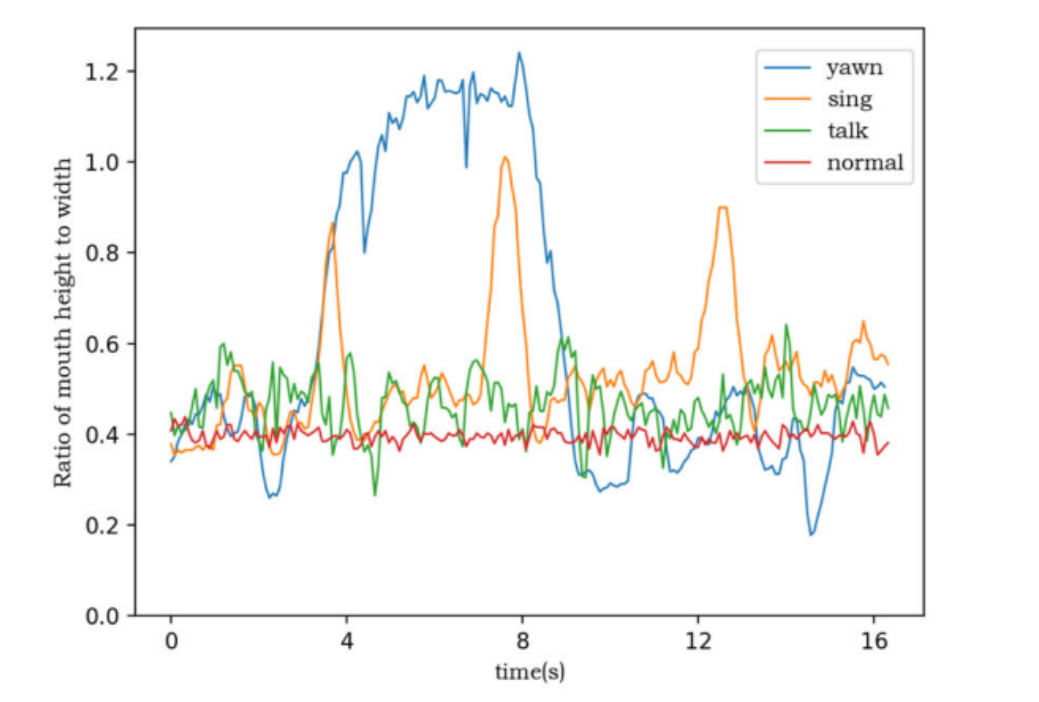
\includegraphics[width=0.5\linewidth]{figures/grafica bostezo.png}
    \caption{Valores de MAR en diferentes estados (\cite{Bostezo})}
    \label{fig:bostezo}
\end{figure}

Experimentación adicional con umbrales de detección de bostezo dieron resultados que indican el valor de 0.5 como el mejor valor de umbral para detección de bostezos a través del MAR, siendo que umbrales de mayores valor daban falsos negativos y menores a 0.5 daban todos falsos positivos. Respecto a la duración total de un bostezo, este dura de 4 a 6 segundos, por lo que un bostezo puede ser establecido como la detección de un valor de mar de 0.5 o mayor durante un lapso de 4 a 6 segundos (\cite{Bostezo}). 




\subsection{Pose de cabeza}
La pose de cabeza se presenta como un indicador secundario de somnolencia, ya que no es necesariamente indicador de somnolencia, y este presenta muchos estados los cuales son irrelevantes para la detección, siendo que solo es de interés cuando el sujeto presente cabeceo, que sucede cuando la cabeza empieza a caerse por su propio peso al quedarse dormido y se levanta al reaccionar ante la caída. 

La estimación de pose de cabeza presenta algunos cálculos y procesos más complejos que las métricas mencionadas anteriormente, debido a que para esta métrica se trata de obtener coordenadas 3D en base a información 2D que presenta la imagen. Existe el algoritmo POSIT que ayuda a cumplir con esta tarea. Sin embargo, es difícil establecer relaciones continuas entre objetos con este algoritmo. Debido a esto, existen múltiples propuestas de cálculos que ayudan a estimar las coordenadas 3D de una imagen 2D, entre estas un algoritmo POSIT adaptado para tareas en tiempo real (\cite{Cabeceo}). 


\section{Detección de distracción}
El uso de redes neuronales convolucionales para la clasificación y detección de distracción está bien documentado a lo largo de investigaciones que hacen uso de bases de datos que contienen imágenes categorizadas en distintos estados de distracción del conductor, así como anotaciones de cuando el conductor está manejando de manera segura. Entre las bases de datos más comúnmente utilizadas para la detección de distracción se encuentran: 

\begin{itemize}
    \item AUC DDD Dataset
    \item State-Farm
    \item Driver Monitoring Dataset
\end{itemize}

La Tabla \ref{tab:distracción} muestra la experimentación realizada en el estado del arte para detección de distracción en un conductor. La tabla muestra una gran variedad de arquitecturas de aprendizaje profundo, así como resultados prometedores en distintas bases de datos. Las dos bases de datos más utilizadas son AUC y State-Farm, donde se obtienen exactitud de hasta 99\% en algunos casos. Solo se presenta una investigación con el uso del conjunto de datos DMD, que obtuvo una exactitud del 73.35\%, lo cual es indicativo de la posible necesidad de arquitecturas complejas para obtener resultados de exactitudes altas. 
\begin{table}[h!]
    \centering
    \footnotesize
    \renewcommand{\arraystretch}{1.8} 
    \begin{tabularx}{\textwidth}{c X X c}
        Investigación & Método de clasificación & Conjunto de datos utilizado & Exactitud \\
        \hline
        \cite{DCNN} & Drive-Net (CNN y Bosque Aleatorio) & Conjunto de datos de Kaggle & 95\% \\
        \cite{Swin} & \textit{Swin Transformer} & AUC-DD y State-Farm & 95.63\% y 99.73\% \\
        \cite{LRCN} &  LCRN & Conjunto de datos propio & 93.9-99.2\% \\
        \cite{D3D} & 3D-CNN & DMD & Exactitud = 73.35\% \\ 
        \cite{CNN-Trans} & CaTNet (ConvNeXt + CaT) & AUC y State-Farm & 94.82\% y 99.91\% \\
        \cite{DyS-VC} & Umbrales cálculados con visión computacional & Posición del iris de los ojos & 89\% \\ 
        \cite{DTF} & AlexNet e InceptionV3 & Conjunto de datos propio & 93.65\% y 95.17\% \\
        \cite{DHM-RNN} & ResNet + HRNN & AUC y State-Farm & 96.23\% y 92.36\% \\
        \hline
    \end{tabularx}
    \caption{Metodología y resultados del estado del arte en detección de distracción}
    \label{tab:distracción}
\end{table}

De acuerdo con el departamento de transporte NHTSA, los automóviles tienen que ser diseñados con el objetivo de que cualquier tarea adicional al manejo tiene que ser completada en un tiempo menor de 2 segundos, siendo así que cualquier actividad de una duración mayor a 2 segundos se considera como una distracción del conductor (\cite{NHTSA}). Este reglamento sirve como una guía absoluta para el establecimiento de la definición de que condiciones deben cumplirse para que algún comportamiento del conductor sea considerado distracción. 

\section{Implementación en tiempo real}

\subsection{\textit{Threading}}
El \textit{Threading} (Hilos de ejecución) es una práctica en la programación de algoritmos en tiempo real que busca dividir las tareas de un programa en múltiples grupos con el objetivo de que estos nuevos subgrupos todos sean ejecutados de manera simultánea, todos sucediendo al mismo tiempo. Esto puede mejorar la eficiencia de las tareas realizadas de un algoritmo, cambiando de un enfoque secuencial a paralelo, evitando de manera especial cuellos de botella en un código y ofreciendo una capacidad de procesamiento mayor. La distribución de tareas ofrece ventajas destacables especialmente cuando se necesita procesar mucha información, por lo cual ofrece una ventaja clara para los sistemas de tiempo real, donde es necesario procesar información, en este caso imágenes, de manera constante y rápida.

Al-sudani et al. llevaron a cabo experimentación de procesamiento de polinomios de Chebyshev utilizando \textit{multithreading}, con el objetivo de comprobar que el uso de \textit{threads} es eficiente, así como encontrar la cantidad de \textit{threads} que mejor optimiza el algoritmo utilizado. Sus resultados dieron conclusiones claras de que la distribución de tareas en diferentes grupos para que se procesen de manera paralela entrega tiempos de ejecución mucho más rápidos, obteniendo una mejora de 7.2 veces mayor velocidad que la versión secuencial (\cite{Threading}). La Figura \ref{fig:threading} muestra resultados de la experimentación realizada por los investigadores, donde las barras rojas representan el tiempo que le tomo al código ejecutarse, los puntos azules la mejoría que presento el código respecto a la secuencia, y el eje x siendo la cantidad de \textit{threads} implementados. Con esta gráfica se puede observar que implementando \textit{threading} con la cantidad de subconjuntos correcta, el tiempo de ejecución de un código disminuye considerablemente. 

\begin{figure}[h!]
    \centering
    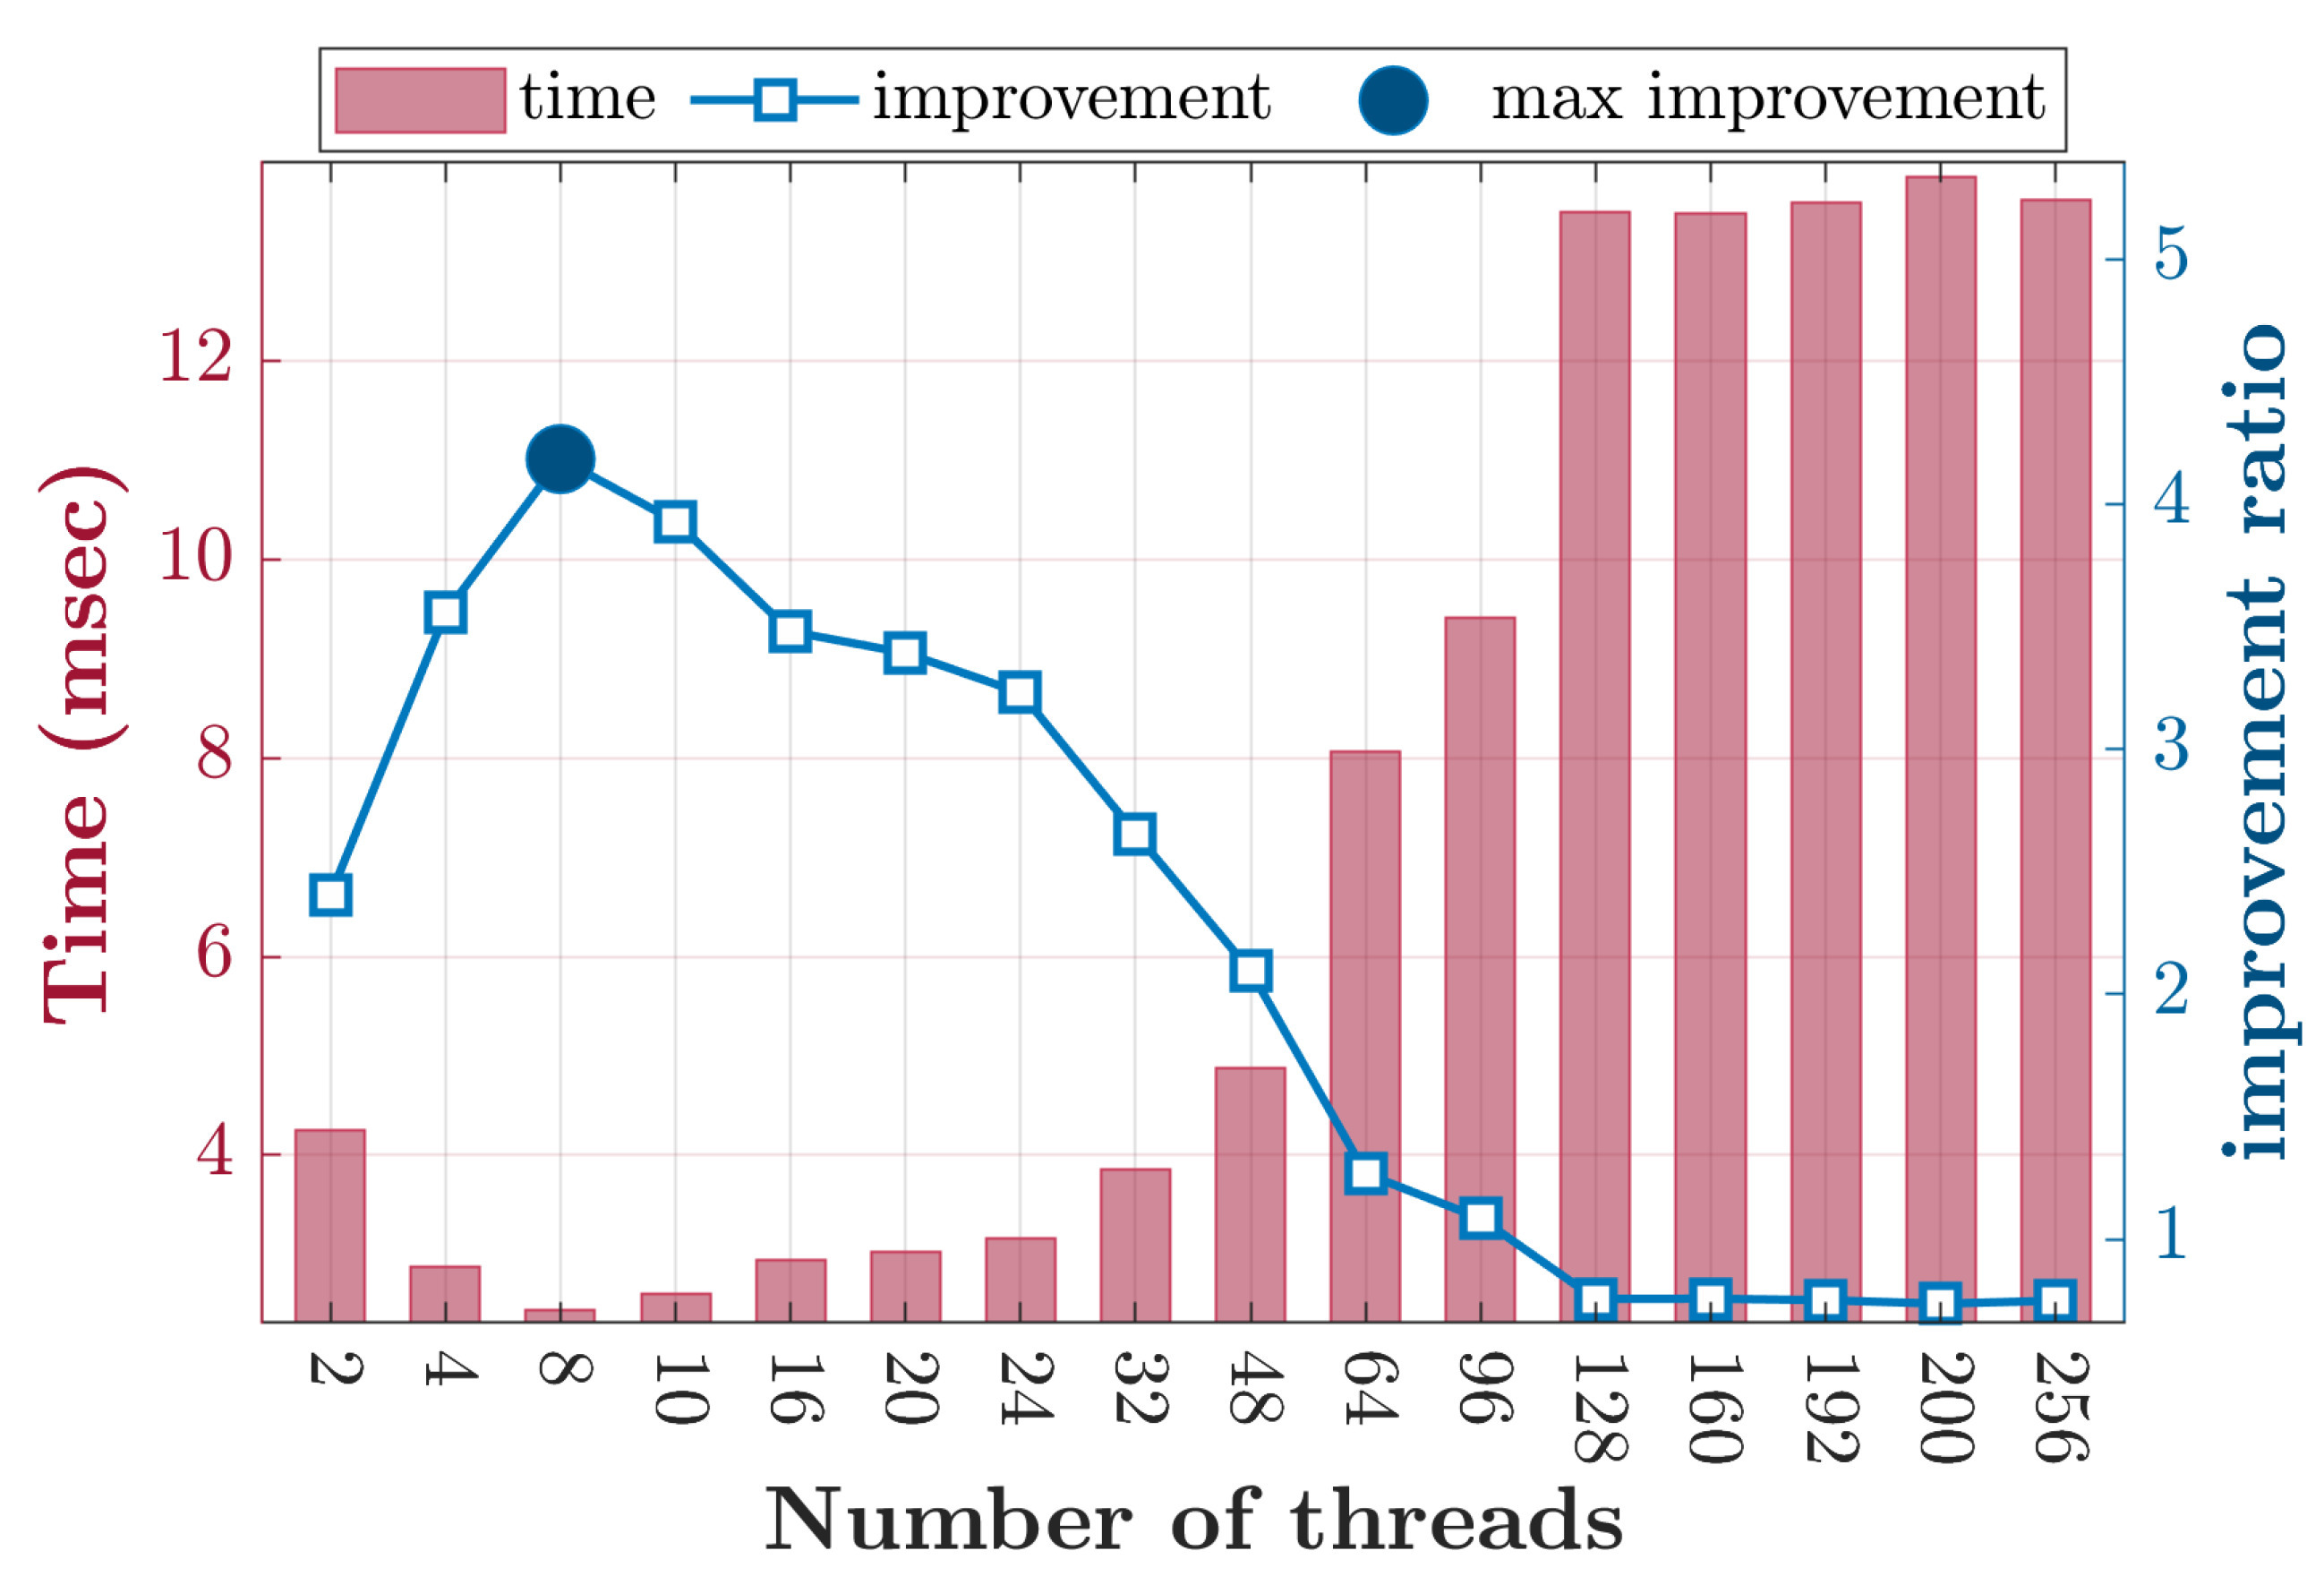
\includegraphics[width=0.5\linewidth]{figures/threading.png}
    \caption{Resultados de uso de \textit{threading} en procesamiento de polinomios de Chevyshev (\cite{Threading})}
    \label{fig:threading}
\end{figure}

\subsection{Comparativa entre lenguajes Python y C++}
El uso de distintos lenguajes en la creación de algoritmos puede traer diferentes ventajas y desventajas dependiendo del lenguaje. Algunos son más interpretables y sencillos de entender, mientras que otros ofrecen mayor velocidad o capacidades de compilación, a costo de interpretabilidad. Estas son precisamente las diferencias que presentan los dos lenguajes utilizados en este trabajo, Python y C++. C++ es un lenguaje que se compila, es decir, lo escrito en el algoritmo se traduce al lenguaje nativo del procesador antes de ser ejecutado. Python no es un lenguaje que se compila, sino que se interpreta, y la diferencia entre este proceso causa que las velocidades de procesamiento entre un lenguaje y otro cambien, siendo C++ el más rápido gracias a la compilación nativa. 

Múltiples investigaciones se han llevado a cabo para probar este fundamento con distintos tipos de tareas y algoritmos en ambos lenguajes. Burda et al. realizan una comparación entre lenguajes respecto a las capacidades que estos presentan para procesar bases de datos de diferentes tamaños, con el objetivo de llegar a una conclusión de cuál es el lenguaje más apto para el procesamiento de datos. Sus resultados demuestran a la perfección que C++ es un lenguaje que supera en velocidad a Python en tareas de procesamiento de datos, obteniendo velocidades mayores en C++ en absolutamente todos los casos de experimentación, presentando también conclusiones de que entre mayor es el conjunto de datos, la diferencia entre velocidades aumenta considerablemente, siendo que Python presenta tiempos mucho más lentos que los que C++ presenta (\cite{C++}). Este comportamiento se puede observar en la Figura \ref{fig:c++}.

\begin{figure}[h!]
    \centering
    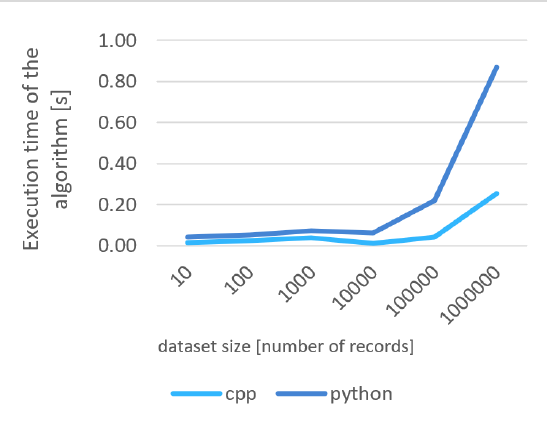
\includegraphics[width=0.5\linewidth]{figures/c++.png}
    \caption{Diferencia de tiempos entre Python y C++ (\cite{C++})}
    \label{fig:c++}
\end{figure}